\documentclass{article}
\usepackage[utf8]{inputenc}
\setlength{\parindent}{0em}
\setlength{\parskip}{1em}
\usepackage[dvipsnames]{xcolor}
\usepackage{hyperref}
\usepackage{minted}
\usepackage{tikz}
\usepackage{amsmath}
\hypersetup{
    colorlinks=true,
    linkcolor=blue,
    filecolor=magenta,
    urlcolor=cyan,
}

\urlstyle{same}

\title{%
Running Osrank on a blockchain \\
\large An informal specification \\
}
\author{
  Di Napoli, Alfredo\\
  \texttt{alfredo@monadic.xyz}
  \and
  Breitkreuz, Merle\\
  \texttt{merle@monadic.xyz}
}

\date{July 2019}

\usepackage{natbib}
\usepackage{graphicx}

\begin{document}

\maketitle

\tableofcontents

\section{Introduction}
\textit{Osrank} is at the heart of the \textit{Oscoin} vision, and is formally defined as \textit{[..]a variant of the well known PageRank algorithm, applied to the graph of relationships between projects and contributions on the network[..]to choose which project receive oscoin and in which proportions.}\citep{opensourcecoin2019}

This document tries to bridge the gap between the theoretical aspect of the paper and the practical one, describing possible ways to implement and run \textit{Osrank} on a blockchain.

\section{User scenarios and requirements}

In this section we present a possible list of user scenarios and requirements for \textit{Osrank}, some of which might fall "in between" the \textit{Osrank} and \textit{Oscoin} projects, but are nevertheless shown here to get a firmer
understanding of the context we are operating in.

\subsection{User scenarios}

In this section, a number of very \textbf{high level} user scenario are
presented. They are vague on purpose; the main aim here is not to figure out
how to do things from a technical perspective, but more to give an eagle-eye
view of how the system should behave.

\subsubsection{Scenario: Node computes Osrank every epoch}

\begin{enumerate}
\item Every \textit{epoch}, i.e. every $k$ blocks, the system runs the
      \textit{Osrank} algorithm.
\item The system gathers the \textit{hyperparameters} and the
      \textit{damping factors} on-chain, from the ledger state.
\item The system loads the actual network graph from an off-chain storage,
      and executes the \textit{Osrank} procedure on it.
\item Each node in the \textit{network graph} has its \textit{Osrank} weight (re-)calculated.
\item A new transaction is created within the system that distributes funds
      from the \textit{Oscoin treasury} to the \textit{graph nodes}, in
      quantity proportional to their \textit{Osrank}.
\end{enumerate}

\subsubsection{Scenario: Oscoin node receives new block with Osrank transaction }

\textit{Nota bene:} We are not going to discuss and address forks in this
scenario, as they simply revert state. We focus on the most common scenario.

\begin{enumerate}
\item A node $N$ receives a new block $B$ from the network
      directly extending $N$'s adopted chain and therefore forming
      the new tip;
\item $N$ verifies each and every transaction in $B$;
\item If one of the transactions $tx$ is a \textit{Osrank} one, the node
      verifies the generated \textit{Osrank} is valid by re-running the
      same computation in a verifiable way;
\item If the verification succeeds, $N$ adds block $B$ as the new tip;
\item If the verification fails, $N$ discards the block $B$ as it
      comes from a potentially malicious network operator.

\end{enumerate}

\subsection{Performance requirements}

\begin{enumerate}
\item The entire \textit{Osrank} algorithm \textit{must} run in
      much less than the \textit{block time}, where for
      \textit{Oscoin} this is set to \textit{60 seconds}.
      A good conservative threshold is for the algorithm to run
      in \textit{50\%} of the total block time, to make sure the
      network operator's node has time to also perform other
      operations, remaining within the same boundary of the
      block time. [Time]
\item The performance of the \textit{Osrank} algorithm shall be
      as much as possible independent from the \textit{size} of the
      network graph. In other terms, having the performance of the
      algorithm be linearly dependent from the size of the graph will
      make it eventually surpass the \textit{block time} hard limit. [Time]
\item The memory allocation of the \textit{Osrank} algorithm must be
      such that it's possible to run the algorithm on most personal
      computers and other devices with limited memory. As most devices
      these days tends to have a RAM of \textit{8 GB}, this seems to be
      a hard limit. [Space]
\end{enumerate}

\subsection{Ledger interface requirements}

\begin{enumerate}
\item It shall be possible to retrieve the
      \textit{hyperparameters}, \textit{damping factors} and
      the values for $R$ and $\tau$ from the
      \textit{Ledger} state, where $R$ is the number
      of random walks to perform for each node $n$ and
      $\tau$ is the pruning threshold for the first
      phase of the algorithm. [Functional]
\item It shall be possible to update the
      \textit{hyperparameters}, \textit{damping factors},
      $R$ and $\tau$ if needed
      (i.e. during a \textit{soft fork}). [Functional]
      \textbf{UPDATE}: This is not relevant to \textit{osrank} directly,
      but obviously it should be possible to update the parameters after
      \textit{mainnet}.
\item If the number of blocks $k$ that determines the length of
      an \textit{epoch} are fixed, it shall be possible to
      get and set $k$ from the \textit{Ledger} state. [Functional]
      \textbf{UPDATE}: This is now stale. This was useful for an approach
      where we would "weight" the contributions based on the age of
      those (for which we would have needed the $k$), but this has
      now been abandoned.
\end{enumerate}

\subsection{Graph API requirements}

\textbf{Nota bene:} This section does not include Ledger-side requirements,
i.e. it doesn't list things like adding/removing nodes or edges from a
network graph, because the \textit{Osrank} algorithm is only concerned
with updating certain \textit{metadata} of a given network topology.
The full list of requirements for the \textit{Graph API} is probably the
union of the \textit{Ledger requirements} and the requirements in
this document.

\begin{enumerate}
\item It shall be possible to execute the \textit{Osrank} algorithm on a
      particular \textit{network graph} with any extra state correctly
      passed to it (e.g the cached \textit{random walks}). [Functional]
\item It shall be possible to modify the weights associated to each
      \textit{edge}, as more \textit{projects} or \textit{accounts} gets
      added. [Functional]
\item It shall be possible to retrieve the \textit{neighbours} associated
      to a particular node in a \textit{network graph}. [Functional]
\item It shall be possible to generate a random-yet-predicable \textit{seed}
      to be used to instantiate a \textit{PRNG} from the \textit{Osrank}
      algorithm, so that the latter is fully deterministic and verifiable.
      [Functional]
\item (\textbf{n.b. Is this a Ledger requirement instead?})
      It shall be possible to retrieve, given a $(k1,k2)$ epoch
      \textit{range}, all the additions/deletions to the network
      graph, so that \textit{Osrank} can use them for the
      incremental algorithm. [Functional]
\end{enumerate}

\subsection{Storage requirements}

\begin{enumerate}
\item It shall be possible to retrieve a \textit{network graph}
      given a unique identifier. [Functional]
\item A \textit{network graph}'s size should not exceed the memory hard
      limit as described in the \textit{Performance Requirements}. [Space]
\end{enumerate}

\section{Challenges and unknowns}

\subsection{Who runs the osrank calculation?}

Status: \textcolor{ForestGreen}{\textbf{Resolved}}

\textbf{Option 1: Native code all the way down}

If this is run by each and every network operator in the system, the only
way to prevent cheating is to have each node in the network validate the output
of the \textit{osrank} algorithm by re-running it against the same state from which
a received block \textit{B} has been created. This also assumes that the algorithm
is cheap to compute. Once the osrank has been calculated, the result must be included
in the new block being mined, alongside with one or more transactions to distribute
the payouts. Here the network operation might need to call into a
smart contract to actually validate the reward transaction, because he/she
wouldn't have the private key to authorise spending from the treasury, so
that needs to come from a "pre-baked" smart contract.

\textbf{Advantages}

\begin{enumerate}
\item Running everything via native code means tapping into the full potential
of a node;
\item No artificial boundaries: hyperparameters \& damping factors are just
      integers/floats, and they are easy to fetch and deserialise from the
      state store, even across an artificial WASM boundary, if any;
\item All the queries on data can happen off-chain, without crossing the
      WASM boundary.
\end{enumerate}

\textbf{Disadvantages}

\begin{enumerate}
\item Not clear how to validate the reward transaction;
\item If the \textit{osrank} computation is not cheap, re-running it for
      validation purposes might be prohibitive.
\end{enumerate}

\textbf{Option 2: WASM code all the way down}

If the osrank algorithm is run on-chain, then the tempting avenue is to have
the osrank algorithm be implemented as a WASM blob/smart contract, which is baked in the genesis block and can be updated via forks. In this scenario
users would create a new transaction every \textit{epoch} (e.g. \textit{k} slots) targeting the smart contract address.

\textbf{Advantages}

\begin{enumerate}
\item Clearer semantic as everything is a smart contract;
\item Generalising this to a graph-ledger might fit naturally within
      this framework;
\item No need to worry about cheating;
\end{enumerate}

\textbf{Disadvantages}

\begin{enumerate}
    \item We might need a gas-model;
    \item We might hit a performance bottleneck when running the algorithm
          via WASM;
    \item Crossing the WASM boundary might be tricky to implement;
\end{enumerate}

\textbf{Resolution}

Out of scope. The scope of this document shouldn't be concerned about technical,
implementation details like WASM. For \textit{Osrank} is sufficient to
know there is a Graph API we can call and that we can rely on the Ledger
to mine a block with the payout.

\subsection{How to generate randomness?}

Status: \textcolor{red}{\textbf{Open}}

In \citep{opensourcecoin2019}, a modification of the algorithm is proposed,
in order to make it resistant to \textit{sybil attacks}. Such modification
involves using a trusted \textit{seed set} from which all the random walks
needs to begin (during the first phase of the algorithm). On top of this,
every time the algorithm visits a node, it has to pick which vertex to
visit next based with a certain probability. In other terms, at every step the
algorithm needs to roll a dice which outcome is biased by the probability on
each edge, but ultimately this step still involves a degree of randomness.

Random functions can usually be seeded which an initial value, in order to
make their evolution deterministic: given an initial seed value, a function
\textit{rand(seed)} will produce a random value alongside a new seed, to be
used in the next call to \textit{rand}.

This naturally give raise to a question: \textit{how to seed the algorithm in a
blockchain context?} Ideally we want to make the output of the algorithm
verifiable and replicable (for obvious reasons) but we do not want
adversaries to be able to "guess" the random walks before the algorithm will
actually run.

\textit{One possibility} as discussed within the team might be to use something
like the hash of the last \textit{k}-blocks to generate a seed, but a bit more
research needs to happen around the robustness of this approach from a
\textit{game theory} perspective: a user might deliberately try to generate
a different seed to generate an \textit{Osrank} which is advantageous to him.

\textbf{Possible Resolution}

Alexis will own this.

\subsection{Is there an initial \texttt{SeedSet} at genesis?}

Status: \textcolor{ForestGreen}{\textbf{Resolved}}

One key characteristic of the \texttt{SeedSet} is that it's composed by a
\textit{trusted} and \textit{curated} collection of projects \& accounts from
which the random walk can be initiated. Therefore, this set must necessarily
be assembled by a trusted party (i.e. like the members of the \textit{oscoin}
project) and distributed on-chain via the genesis block.

\textbf{Resolution}

Due to the fact the initial set of projects will be limited to the ones that
decide to be early adopter of \textit{Oscoin}, the process could be curated
by \textit{Monadic GmbH} itself.

\subsection{Do we need to update the \texttt{SeedSet} periodically, and how?}

Status: \textcolor{ForestGreen}{\textbf{Resolved}}

The main insight behind the \textit{seed set} is to make sure eventually the
random walks explore the totality of the network graph, including disconnected
components. It's conceivable that as more projects gets added, the more the
initial \textit{seed set} will be out-of-date, and in need of an update.

\textbf{Resolution}

Out of the scope.

\subsection{Should we store \texttt{R}, \texttt{k} and the \texttt{TrustRank} threshold on the Ledger?}

Status: \textcolor{ForestGreen}{\textbf{Resolved}}

In the incremental MonteCarlo implementation, the parameter $R$ is used as a
coefficient to calculate the final rank, in the approximated formula. Conversely,
we define that the system enters a new \textit{epoch} every $k$ blocks. Last but
not least, \textit{TrustRank} (from which the \textit{seed set} idea is taken) uses
a \textit{threshold} parameter to prune the initial network graph before running the
"real" algorithm.

Should we store these parameters on the Ledger or should these be hardcoded?

\textbf{Resolution}

On Ledger, not sure yet about $k$ but not relevant for Osrank team we will
have this info.

\subsection{Is there an initial network graph at genesis?}

Status: \textcolor{ForestGreen}{\textbf{Resolved}}

If there is an initial seed set, it's quite likely there will be an initial
network which will be baked into the genesis block. Not doing that means that
there will be some project/accounts in the seed set referencing non-existing
nodes inside the network graph, and this could potentially be an invariant
violation, as the \textit{TrustRank} algorithm requires the seed set to
reference valid nodes.

Are we OK with a genesis block which could be potentially hundreds of megabytes?

\textbf{Resolution}

We won't need to include entire ecosystems into genesis, but likely only
the number of projects and accounts which would sign as early adopters. This
means that, in practice, the initial network graph, especially if compressed,
shouldn't be too big, probably in the ballpark of 3-4 MB, if we
consider the possibility to add \textit{metadata}.

\subsection{How can a network operator verify the osrank (incremental) computation without the remote's cached random walks?}

Status: \textcolor{ForestGreen}{\textbf{Resolved}}

One of the suggested improvement described in \citep{opensourcecoin2019} is
the use of an incremental algorithm based on the work of
\citep{bahmani10pagerank}. This algorithm uses a set of cached random walks
to compute the osrank incrementally and in a fast manner. However, this
poses a challenge for \textit{verifying} the algorithm, because the set of
cached random walks of the \textit{verifier} will be probably different from
the one of the node which originally computed the osrank.

One obvious solution would be to
\textit{store the set of random walks on chain} as part of the output of the
osrank calculation, assuming the size of such walks is such that storing this
as part of the Ledger state is feasible.

\textbf{Resolution}

If the algorithm is deterministic and it is seeded with a PRNG, and all miners
use the same source of entropy, then theoretically the set of random walks
should be predictable and deterministic as well. In terms of \textit{where}
to store the cached information, the most feasible place is on secondary
memory (i.e. disk), as doing so on the \textit{Ledger} would take too much
space. Note that this means that network operations might miss some
information if they have been offline for too long or simply new to the
network. In either cases, the node syncing algorithm can solve both
concerns: during syncing a set of random walks would be generate every
\textit{epoch}.

N.B The cache/storage will need to be thought through
(possibly between Osrank \& Protocol team).

\subsection{How to distribute oscoin to accounts in a graph?}

Status: \textcolor{YellowOrange}{\textbf{Resolving}}

The paper computes the \textit{osrank} for projects \textit{and} accounts,
so it might seem spontaneous to include some form of payouts to these accounts
as well, as "influential" members of the network. If this is a viable venue,
then the shape of a reward transaction should be different from the one
described in the paper, which distributes funds associated to a project's
smart contract.

Resolution: Ledger \& Protocol team will design this
\& will require Osrank to somehow either supply these
rankings out of the algorithm calculation or as
part of the storage.

\subsection{What is the shape of an osrank transaction?}

Status: \textcolor{ForestGreen}{\textbf{Resolved}}

A question which arise spontaneously is how big an "osrank transaction" should
be. Ideally speaking, once the \textit{osrank} has been calculated (for each
project in the network) such up-to-date values are transmitted on-chain by
forging a new, big transaction which informs the ledger that the osranks
have changed. If this is true, how big such transaction will be? The number
of projects and accounts is unbound, so the size of such transaction will
grow linearly with the size of the ecosystem, which is not ideal.

Resolution: no need for transaction because the
concept of osrank is intrisic to the protocol.

\subsection{What is the shape of a reward transaction?}

Status: \textcolor{ForestGreen}{\textbf{Resolved}}

Similarly to the question above, a genuine question is what should be the
shape of a reward transaction. According to \citep{opensourcecoin2019}, there
should be "[..]a reward in \textit{oscoin} which is derived from each project's
\textit{osrank} and distributed via the project's associated smart
contract[..]"

This seems to suggest the existence of a single, enormous transaction where
the \textit{inputs} are the smart contracts of each project in the network
(for which the \textit{Osrank} has been computed) and as output the output of these
contracts, which is one or more \textit{addresses} that will need to receive
\textit{oscoin}. How big such transaction will be?

\textbf{Resolution}

Although it's not fully clear how things will work on the smart contract/
Ledger side (but that's outside the scope of this document) in the
implementation there will be no \textit{treasury} in the common Blockchain
sense, but rather the \textit{coinbase reward} $B_r$ will be bigger every
$k$ blocks (i.e. bigger for the block in which the \textit{Osrank}
is (re-)calculated) which will avoid any complication stemming from
implementing a proper \textit{treasury}.

\subsection{Where to store the cached random walks?}

Status: \textcolor{red}{\textbf{Open}}

In \citep{bahmani10pagerank}, the random walks were stored in an ad-hoc, in-house
NoSQL graph database (i.e. \textit{FlockDB}, now unmaintained). We should discuss
storage options.

\textbf{Possible resolution}

Neo4J or custom storage? Requires more research.

\subsection{How to deal with the Graph's disconnected components?}

Status: \textcolor{ForestGreen}{\textbf{Resolved}}

The full network graph is, in reality, composed by a certain number of
disconnected components. Think, for example, to a "Haskell" component and a
"Rust" component: even though some `Account` might be contributing to projects
in both ecosystems, it's likely that the Rust's projects and Haskell's project
won't have a single link between them. This poses a number of interesting questions:

\begin{enumerate}
\item How does this influence the random walks?
\item Hoes does influence the final \textit{Osrank} calculation? How much
      does it "dilute" it?
\end{enumerate}

\textbf{Possible resolution}

In theory disconnected components shouldn't be a problem. The initial
walk originated from the seed sets should help cutting nodes which have a
way-too-low \textit{Osrank} so that the will receive an \textit{Osrank} of
$0$ at the end. This will help with the "dilution".

\subsection{Should $Osrank$ be modeled as a f64? }

Status: \textcolor{red}{\textbf{Open}}

In order to verify the \textit{Osrank} calculation, it's paramount that all the
network operators (re)running the algorithm would get the same result, which means
the same (updated) set of random walks and all the ranks. However, if the
\textit{Osrank} is calculated as a floating point (i.e. a Rust `f64`) this might be
problematic / bordeline dangerous for two reasons:

\begin{enumerate}
\item Apparently IEEE floating point numbers are interpreted differently according
      to different architectures;
\item We might be subject to rounding errors, so the final probability distribution
      won't sum to 1.0 eventually.
\end{enumerate}

To demonstrate this is a concern, the IOHK folks wrote
a \href{https://hydra.iohk.io/build/902266/download/1/non-integer-calculations.pdf}{specification} on how to deal with non-integral calculations.

\textbf{Resolution}

None yet. Exploring \href{http://www.johngustafson.net/pdfs/BeatingFloatingPoint.pdf}{posits} might be interesting. There is also a \href{https://hal.inria.fr/hal-01959581v2/document}{review} from
INRIA. The downside of \textit{posits} seems to be that the
precision depends on the scale of the operations. This might pose
a problem for things like \textit{Osrank} itself, which is
modeled as a probability distribution.

\subsection{ What should happen if a completely isolated node is added to the graph? }

Status: \textcolor{ForestGreen}{\textbf{Resolved}}

The incremental Monte Carlo paper defines the approximated \textit{PageRank} this way:

$$
\pi_u = \frac{X_u}{\frac{nR}{\epsilon}}
$$

This technically means that from a mathematical standpoint, if $n$ grows (because a new
node has been added to the graph) then the rank for \textit{all} the affected nodes
will need to change. However, from an intuitive point of view, when adding a new project,
if this project doesn't have any incoming edges, it means it has no value for the
community. Not only that, but it could be effectively used as an attack vector, to slow
down the overall \textit{Osrank} calculation. However, the \textit{pruning} via the
\textit{seed set} will ensure that eventually these new node is disregarded during the
real calculation, as its rank is $0$ and therefore it doesn't meet the threshold
requirement.

\textbf{Resolution}

Osrank is set to 0 for those, and we can skip it.
Insight: if a node is not connected to one of the seed
set nodes is not reachable.

\subsection{ Should we have to deal with the added complexity of multiple project versions? }

Status: \textcolor{red}{\textbf{Open}}

The \textit{Osrank} algorithm runs under performance hard-limits (i.e. time to compute
way less than the \textit{block time}) and therefore anything which adds complexity
should be avoided. More specifically, incorporating the concept of project versions poses
quite a few challenges to the \textit{Osrank} team:

\begin{enumerate}
\item If a project has on average 10 versions (and that's optimistic) we might be
      looking (in the worst case scenario) to a 10x increase in the graph size, even
      though is conceivable most projects would depend only from the top 3-4 newest
      project versions.
\item The \textit{Osrank} incremental algorithm needs to (re)compute the random walks
      every time an edge is added \textit{or} removed from the graph: not
      \textit{all} the walks need an update, but only for the ones for which
      contained the updated node (i.e. a node "impacted" by the edge removal). If we
      allow checkpoints to take into account versions, upon a version dump it's
      conceivable three things are going to happen: a new node (for the version) is added
      (either at checkpointing or previously), a new edge is created from the project to
      the \textit{new} version and an edge is \textit{removed} from the project to the
      old version. This might create more work for the \textit{Osrank} algorithm, which
      might make it exceed the hard-limit threshold.
\end{enumerate}

\textbf{Resolution}

None yet.

\section{The Osrank Basic Model}

This section outlines the basic \textit{osrank} model described in the oscoin whitepaper
\url{http://oscoin.io/oscoin.pdf} in a more practical way to create a common
understanding of its functionality. In particular it documents how the adjacency
matrix is constructed which then can be fed into a PageRank algorithm. The latter
will (for now) not be described in detail. At a later point this document should
be expanded to describe the full \textit{osrank} algorithm.

\subsection{Create the adjacency matrix}
\subsubsection{By-hand via-graph approach}

\noindent We start with a directed graph of projects $P$ and Accounts $A$.
Dependencies (depend/d) are edges between projects. Edges between accounts and
projects are always in both directions. They represent contributions (contrib/c)
and maintainers (maintain/m).

\begin{center}
  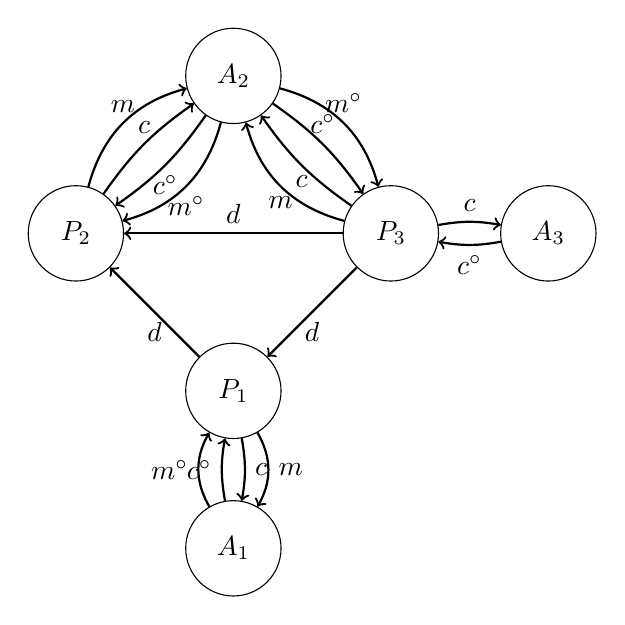
\begin{tikzpicture}[vertex/.style={draw,circle,minimum width=8ex}, arr/.style={draw,thick,->}]
    \node[vertex] (pone) at (0,-2)  {$P_1$};
    \node[vertex] (ptwo) at (-2,0) {$P_2$};
    \node[vertex] (pthree) at (2,0) {$P_3$};
    \node[vertex] (aone) at (0,-4) {$A_1$};
    \node[vertex] (atwo) at (0,2) {$A_2$};
    \node[vertex] (athree) at (4,0) {$A_3$};

    \draw[arr] (pone) edge node[below] {$d$} (ptwo);
    \draw[arr] (pthree) edge node[above] {$d$} (ptwo);
    \draw[arr] (pthree) edge node[below] {$d$} (pone);
    \draw[arr] (athree) to[out=190, in=-10] node[below] {$c^\circ$} (pthree);
    \draw[arr] (pthree) to[out=10, in=170] node[above] {$c$} (athree);

    \draw[arr] (aone) to[out=100, in=-100] node[left] {$c^\circ$} (pone);
    \draw[arr] (pone) to[out=-80, in=80] node[right] {$c$} (aone);
    \draw[arr] (aone) to[out=120, in=-120] node[left] {$m^\circ$} (pone);
    \draw[arr] (pone) to[out=-60, in=60] node[right] {$m$} (aone);

    \draw[arr] (atwo) to[out=-125, in=35] node[below] {$c^\circ$} (ptwo);
    \draw[arr] (ptwo) to[out=55, in=-145] node[above] {$c$} (atwo);
    \draw[arr] (atwo) to[out=-105, in=15] node[below] {$m^\circ$} (ptwo);
    \draw[arr] (ptwo) to[out=75, in=-165] node[above] {$m$} (atwo);

    \draw[arr] (atwo) to[out=-35, in=125] node[above] {$c^\circ$} (pthree);
    \draw[arr] (pthree) to[out=145, in=-55] node[below] {$c$} (atwo);
    \draw[arr] (atwo) to[out=-15, in=105] node[above] {$m^\circ$} (pthree);
    \draw[arr] (pthree) to[out=165, in=-75] node[below] {$m$} (atwo);
  \end{tikzpicture}
\end{center}

\noindent In the first step, each edge will be weighted according to their type.

\begin{center}
  \begin{tabular}{ |c|c| }
    \hline
    edge type & value \\
    \hline
    $depend$ & $\frac{4}{7}$ \\
    \hline
    $contrib$ & $\frac{1}{7}$ \\
    \hline
    $maintain$ & $\frac{2}{7}$ \\
    \hline
    $contrib^\circ$ & $\frac{2}{5}$ \\
    \hline
    $maintain^\circ$ & $\frac{3}{5}$ \\
    \hline
  \end{tabular}
  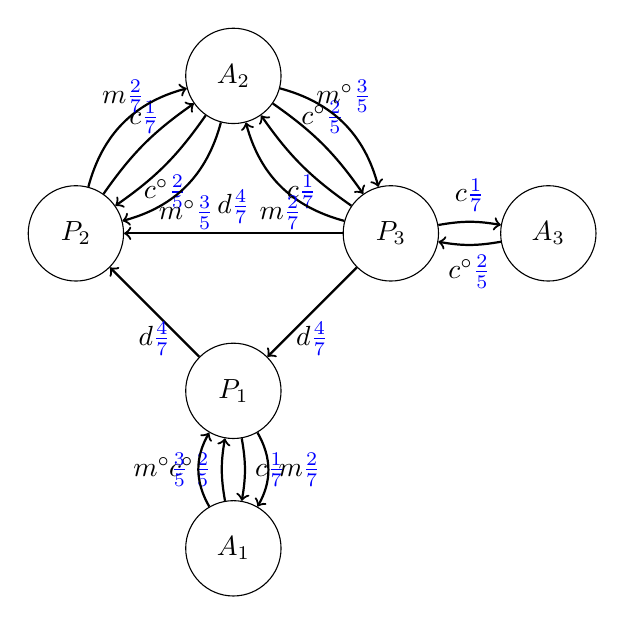
\begin{tikzpicture}[vertex/.style={draw,circle,minimum width=8ex}, arr/.style={draw,thick,->}]
    \node[vertex] (pone) at (0,-2)  {$P_1$};
    \node[vertex] (ptwo) at (-2,0) {$P_2$};
    \node[vertex] (pthree) at (2,0) {$P_3$};
    \node[vertex] (aone) at (0,-4) {$A_1$};
    \node[vertex] (atwo) at (0,2) {$A_2$};
    \node[vertex] (athree) at (4,0) {$A_3$};

    \draw[arr] (pone) edge node[below] {$d \textcolor{blue}{\frac{4}{7}}$} (ptwo);
    \draw[arr] (pthree) edge node[above] {$d \textcolor{blue}{\frac{4}{7}}$} (ptwo);
    \draw[arr] (pthree) edge node[below] {$d \textcolor{blue}{\frac{4}{7}}$} (pone);
    \draw[arr] (athree) to[out=190, in=-10] node[below] {$c^\circ \textcolor{blue}{\frac{2}{5}}$} (pthree);
    \draw[arr] (pthree) to[out=10, in=170] node[above] {$c \textcolor{blue}{\frac{1}{7}}$} (athree);

    \draw[arr] (aone) to[out=100, in=-100] node[left] {$c^\circ \textcolor{blue}{\frac{2}{5}}$} (pone);
    \draw[arr] (pone) to[out=-80, in=80] node[right] {$c \textcolor{blue}{\frac{1}{7}}$} (aone);
    \draw[arr] (aone) to[out=120, in=-120] node[left] {$m^\circ \textcolor{blue}{\frac{3}{5}}$} (pone);
    \draw[arr] (pone) to[out=-60, in=60] node[right] {$m \textcolor{blue}{\frac{2}{7}}$} (aone);

    \draw[arr] (atwo) to[out=-125, in=35] node[below] {$c^\circ \textcolor{blue}{\frac{2}{5}}$} (ptwo);
    \draw[arr] (ptwo) to[out=55, in=-145] node[above] {$c \textcolor{blue}{\frac{1}{7}}$} (atwo);
    \draw[arr] (atwo) to[out=-105, in=15] node[below] {$m^\circ \textcolor{blue}{\frac{3}{5}}$} (ptwo);
    \draw[arr] (ptwo) to[out=75, in=-165] node[above] {$m \textcolor{blue}{\frac{2}{7}}$} (atwo);

    \draw[arr] (atwo) to[out=-35, in=125] node[above] {$c^\circ \textcolor{blue}{\frac{2}{5}}$} (pthree);
    \draw[arr] (pthree) to[out=145, in=-55] node[below] {$c \textcolor{blue}{\frac{1}{7}}$} (atwo);
    \draw[arr] (atwo) to[out=-15, in=105] node[above] {$m^\circ \textcolor{blue}{\frac{3}{5}}$} (pthree);
    \draw[arr] (pthree) to[out=165, in=-75] node[below] {$m \textcolor{blue}{\frac{2}{7}}$} (atwo);
  \end{tikzpicture}
\end{center}

\noindent The whitepaper then suggests to adjust these weights again.
The values of $depend$  and $maintain$ are each divided by the corresponding
count of outgoing edges of the same type on the node.
$contrib^\circ$ and $maintain^\circ$ are multiplied by the number of
contributions of the account to the project, divided by the total number of
contributions of the account. $contrib$ is multiplied by the number of
contributions of the account to the project, divided by the total number of
contributions in the project.\\
In the graph below, information about the number of contributions for each
connection is represented by the red number in the squares. Factors of value $1$
are omitted. This occurs if the node has only one outgoing edge of the same type.

\begin{center}
  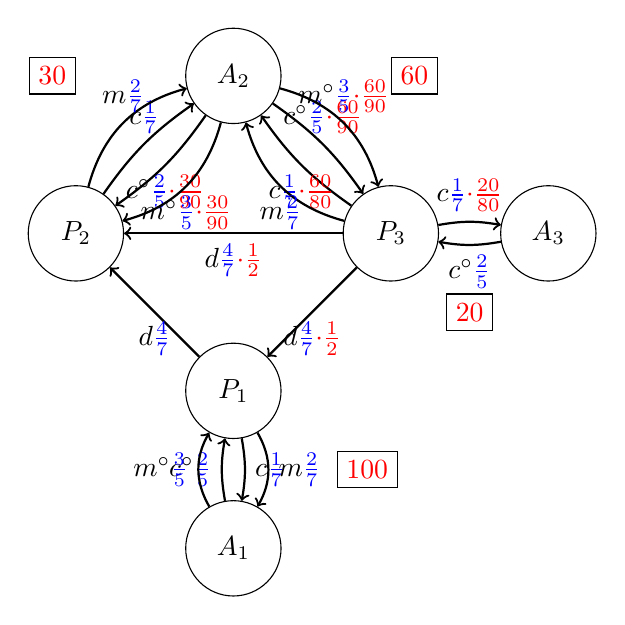
\begin{tikzpicture}[vertex/.style={draw,circle,minimum width=8ex}, arr/.style={draw,thick,->}]
    \node[vertex] (pone) at (0,-2)  {$P_1$};
    \node[vertex] (ptwo) at (-2,0) {$P_2$};
    \node[vertex] (pthree) at (2,0) {$P_3$};
    \node[vertex] (aone) at (0,-4) {$A_1$};
    \node[vertex] (atwo) at (0,2) {$A_2$};
    \node[vertex] (athree) at (4,0) {$A_3$};

    \node[draw] at (-2.3,2) {$\textcolor{red}{30}$};
    \node[draw] at (3,-1) {$\textcolor{red}{20}$};
    \node[draw] at (2.3,2) {$\textcolor{red}{60}$};
    \node[draw] at (1.7,-3) {$\textcolor{red}{100}$};

    \draw[arr] (pone) edge node[below] {$d \textcolor{blue}{\frac{4}{7}}$} (ptwo);
    \draw[arr] (pthree) edge node[below] {$d \textcolor{blue}{\frac{4}{7}}\textcolor{red}{\cdot\frac{1}{2}}$} (ptwo);
    \draw[arr] (pthree) edge node[below] {$d \textcolor{blue}{\frac{4}{7}}\textcolor{red}{\cdot\frac{1}{2}}$} (pone);
    \draw[arr] (athree) to[out=190, in=-10] node[below] {$c^\circ \textcolor{blue}{\frac{2}{5}}$} (pthree);
    \draw[arr] (pthree) to[out=10, in=170] node[above] {$c \textcolor{blue}{\frac{1}{7}}\textcolor{red}{\cdot\frac{20}{80}}$} (athree);

    \draw[arr] (aone) to[out=100, in=-100] node[left] {$c^\circ \textcolor{blue}{\frac{2}{5}}$} (pone);
    \draw[arr] (pone) to[out=-80, in=80] node[right] {$c \textcolor{blue}{\frac{1}{7}}$} (aone);
    \draw[arr] (aone) to[out=120, in=-120] node[left] {$m^\circ \textcolor{blue}{\frac{3}{5}}$} (pone);
    \draw[arr] (pone) to[out=-60, in=60] node[right] {$m \textcolor{blue}{\frac{2}{7}}$} (aone);

    \draw[arr] (atwo) to[out=-125, in=35] node[below] {$c^\circ \textcolor{blue}{\frac{2}{5}}\textcolor{red}{\cdot\frac{30}{90}}$} (ptwo);
    \draw[arr] (ptwo) to[out=55, in=-145] node[above] {$c \textcolor{blue}{\frac{1}{7}}$} (atwo);
    \draw[arr] (atwo) to[out=-105, in=15] node[below] {$m^\circ \textcolor{blue}{\frac{3}{5}}\textcolor{red}{\cdot\frac{30}{90}}$} (ptwo);
    \draw[arr] (ptwo) to[out=75, in=-165] node[above] {$m \textcolor{blue}{\frac{2}{7}}$} (atwo);

    \draw[arr] (atwo) to[out=-35, in=125] node[above] {$c^\circ \textcolor{blue}{\frac{2}{5}}\textcolor{red}{\cdot\frac{60}{90}}$} (pthree);
    \draw[arr] (pthree) to[out=145, in=-55] node[below] {$c \textcolor{blue}{\frac{1}{7}}\textcolor{red}{\cdot\frac{60}{80}}$} (atwo);
    \draw[arr] (atwo) to[out=-15, in=105] node[above] {$m^\circ \textcolor{blue}{\frac{3}{5}}\textcolor{red}{\cdot\frac{60}{90}}$} (pthree);
    \draw[arr] (pthree) to[out=165, in=-75] node[below] {$m \textcolor{blue}{\frac{2}{7}}$} (atwo);
  \end{tikzpicture}
\end{center}

\noindent Finally we want to reduce the graph to single edges only, so $maintain$
and $contrib$ and $contrib^\circ$ and $maintain^\circ$ are summed up. The weights
of outgoing edges are then normalized per node to ensure that all outgoing edge
weights of one node add up to 1.

\begin{center}
  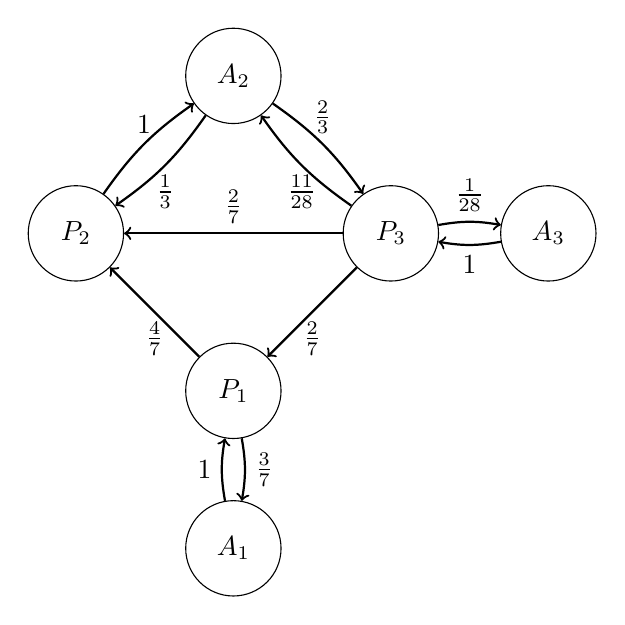
\begin{tikzpicture}[vertex/.style={draw,circle,minimum width=8ex}, arr/.style={draw,thick,->}]
    \node[vertex] (pone) at (0,-2)  {$P_1$};
    \node[vertex] (ptwo) at (-2,0) {$P_2$};
    \node[vertex] (pthree) at (2,0) {$P_3$};
    \node[vertex] (aone) at (0,-4) {$A_1$};
    \node[vertex] (atwo) at (0,2) {$A_2$};
    \node[vertex] (athree) at (4,0) {$A_3$};

    \draw[arr] (pone) edge node[below] {$\frac{4}{7}$} (ptwo);
    \draw[arr] (pthree) edge node[above] {$\frac{2}{7}$} (ptwo);
    \draw[arr] (pthree) edge node[below] {$\frac{2}{7}$} (pone);
    \draw[arr] (athree) to[out=190, in=-10] node[below] {$1$} (pthree);
    \draw[arr] (pthree) to[out=10, in=170] node[above] {$\frac{1}{28}$} (athree);

    \draw[arr] (aone) to[out=100, in=-100] node[left] {$1$} (pone);
    \draw[arr] (pone) to[out=-80, in=80] node[right] {$\frac{3}{7}$} (aone);

    \draw[arr] (atwo) to[out=-125, in=35] node[below] {$\frac{1}{3}$} (ptwo);
    \draw[arr] (ptwo) to[out=55, in=-145] node[above] {$1$} (atwo);

    \draw[arr] (atwo) to[out=-35, in=125] node[above] {$\frac{2}{3}$} (pthree);
    \draw[arr] (pthree) to[out=145, in=-55] node[below] {$\frac{11}{28}$} (atwo);
  \end{tikzpicture}
\end{center}

\noindent The final graph can be represented in a adjacency matrix.
\begin{center}
  \begin{tabular}{c | c c c c c c c}
    & $P_1$ & $P_2$ & $P_3$ & $A_1$ & $A_2$ & $A_3$ \\
    \hline
    $P_1$ & 0 & $\frac{4}{7}$ & 0 & $\frac{3}{7}$ & 0 & 0 \\
    $P_2$ & 0 & 0 & 0 & 0 & 1 & 0 \\
    $P_3$ & $\frac{2}{7}$ & $\frac{2}{7}$ & 0 & 0 & $\frac{11}{28}$ & $\frac{1}{28}$ \\
    $A_1$ & 1 & 0 & 0 & 0 & 0 & 0 \\
    $A_2$ & 0 & $\frac{1}{3}$ & $\frac{2}{3}$ & 0 & 0 & 0 \\
    $A_3$ & 0 & 0 & 1 & 0 & 0 & 0 \\
  \end{tabular}
\end{center}

\subsubsection{Via-dataset approach}
For this approach we divide the final adjacency matrix into 4 quadrants and
calculate each quadrant separately.
\begin{center}
  \begin{math}
    \left(
    \begin{array}{ c|c }
      P\rightarrow P & P\rightarrow A \\
      \hline
      A\rightarrow P & A\rightarrow A \\
    \end{array}
    \right)
  \end{math}
\end{center}
We start off with 3 matrices constructed out of provided data. Note that the
order of projects and accounts has to be consistent for each matrix. $D$ is the
dependency adjacency matrix with values $0$ or $1$ representing dependencies of
projects. $C$ is the contributions adjacency matrix with values $0$ or the number
of contributions the account made to the specific project. $M$ is the maintainers
adjacency matrix with values $0$ or $1$. For $C$ and $M$ the rows represent the
projects and the columns the accounts.\\
For the example above, the matrices would look like this:
\begin{displaymath}
  D =
  \begin{pmatrix}
    0 & 1 & 0 \\
    0 & 0 & 0 \\
    1 & 1 & 0 \\
  \end{pmatrix}
  , C =
  \begin{pmatrix}
    100 & 0 & 0 \\
    0 & 30 & 0 \\
    0 & 60 & 20 \\
  \end{pmatrix}
  , M =
  \begin{pmatrix}
    1 & 0 & 0 \\
    0 & 1 & 0 \\
    0 & 1 & 0 \\
  \end{pmatrix}
\end{displaymath}
These adjacency matrices together with the initial and additional factors are
then used to calculate the quadrants. The $A\rightarrow A$ quadrant is just a
matrix of zeroes as there are no connections between accounts.
\begin{align*}
  P\rightarrow P &= d \cdot norm_{row}(D) \\
  P\rightarrow A &= m \cdot norm_{row}(M) + c\cdot norm_{row}(C) \\
  A\rightarrow P &= ((m^{\circ}\cdot M^T) \odot norm_{row}(C^T)) + c^{\circ}\cdot norm_{row}(C^T)
\end{align*}
where $\odot$ is the Hadamat product and $norm_{row}$ is the row-wise
normalization.\\
Combining all quadrants as represented above and applying $norm_{row}$ again to
the final matrix, results in the same adjacency matrix as at the end of the last
section.
\subsection{Customized PageRank}
\subsubsection{Naive Osrank}
The static \textit{osrank} model runs a customized PageRank algorithm on
the weighted directed graph constructed in the last section.
The only customization for now is the addition of damping factors.
The factor is the probability that a random walk will continue.
For \textit{osrank} we distinguish between damping factors for projects
$\epsilon_{project}$ and accounts $\epsilon_{account}$. So for example
$1-\epsilon_{project}$ refers to the probability that the random walk will
terminate on a project node.\\
The values for the factors were not further specified in the whitepaper, for
classic PageRank implementation often a damping factor of $0.85$ is used.

\subsubsection{Monte Carlo Random walks}
In this approach the \textit{osrank} is calculated by doing $R$ random walks
starting from each node of the graph. The rank for a node $x$ is then derived by:

\begin{displaymath}
  \omega(x) = \frac{W_x (1-\epsilon_{node})}{n R}
\end{displaymath}

where $n$ is the number of nodes in the graph and $W_x$ is the number of visits
to $x$ of all random walks.\\
The random walks can either be made on a pre-weighted graph as described above,
or weighing the edges can happen on the fly while walking on the graph. For
this, the graph has to be constructed slightly different, which will be
described here.\\
In this graph, edge types are not collapsed into each other to end up with a
graph with single edges as above. Here, each node has at most one edge of the same
type. The number of contributions which influences the weights of $c$,
$c^{\circ}$ and $m^{\circ}$ is stored in counters on those edges. $d$ and $m$ do
not need counters.\\

\begin{center}
  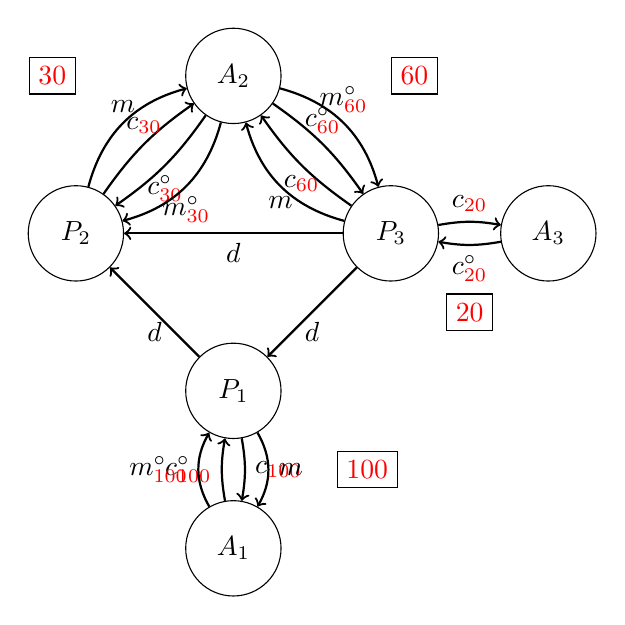
\begin{tikzpicture}[vertex/.style={draw,circle,minimum width=8ex}, arr/.style={draw,thick,->}]
    \node[vertex] (pone) at (0,-2)  {$P_1$};
    \node[vertex] (ptwo) at (-2,0) {$P_2$};
    \node[vertex] (pthree) at (2,0) {$P_3$};
    \node[vertex] (aone) at (0,-4) {$A_1$};
    \node[vertex] (atwo) at (0,2) {$A_2$};
    \node[vertex] (athree) at (4,0) {$A_3$};

    \node[draw] at (-2.3,2) {$\textcolor{red}{30}$};
    \node[draw] at (3,-1) {$\textcolor{red}{20}$};
    \node[draw] at (2.3,2) {$\textcolor{red}{60}$};
    \node[draw] at (1.7,-3) {$\textcolor{red}{100}$};

    \draw[arr] (pone) edge node[below] {$d$} (ptwo);
    \draw[arr] (pthree) edge node[below] {$d$} (ptwo);
    \draw[arr] (pthree) edge node[below] {$d$} (pone);
    \draw[arr] (athree) to[out=190, in=-10] node[below] {$c^\circ_{\textcolor{red}{20}}$} (pthree);
    \draw[arr] (pthree) to[out=10, in=170] node[above] {$c_{\textcolor{red}{20}}$} (athree);

    \draw[arr] (aone) to[out=100, in=-100] node[left] {$c^\circ_{\textcolor{red}{100}}$} (pone);
    \draw[arr] (pone) to[out=-80, in=80] node[right] {$c_{\textcolor{red}{100}}$} (aone);
    \draw[arr] (aone) to[out=120, in=-120] node[left] {$m^\circ_{\textcolor{red}{100}}$} (pone);
    \draw[arr] (pone) to[out=-60, in=60] node[right] {$m$} (aone);

    \draw[arr] (atwo) to[out=-125, in=35] node[below] {$c^\circ_{\textcolor{red}{30}}$} (ptwo);
    \draw[arr] (ptwo) to[out=55, in=-145] node[above] {$c_{\textcolor{red}{30}}$} (atwo);
    \draw[arr] (atwo) to[out=-105, in=15] node[below] {$m^\circ_{\textcolor{red}{30}}$} (ptwo);
    \draw[arr] (ptwo) to[out=75, in=-165] node[above] {$m$} (atwo);

    \draw[arr] (atwo) to[out=-35, in=125] node[above] {$c^\circ_{\textcolor{red}{60}}$} (pthree);
    \draw[arr] (pthree) to[out=145, in=-55] node[below] {$c_{\textcolor{red}{60}}$} (atwo);
    \draw[arr] (atwo) to[out=-15, in=105] node[above] {$m^\circ_{\textcolor{red}{60}}$} (pthree);
    \draw[arr] (pthree) to[out=165, in=-75] node[below] {$m$} (atwo);
  \end{tikzpicture}
\end{center}

To choose the next node for the random walk from node $N_i$, first the type of
edge is chosen, weighted by the hyperparams. Then for $d$ and $m$ the next edge
is chosen equiprobable. For $c$, $c^{\circ}$ and $m^{\circ}$ each edge is
weighted by the number of contributions of the edge, normalized by the total
number of contributions of $N_i$. (Note: $SliceRandom::choose\_weighted$ in
Rust normalizes all weights, so that passing the counter for each edge is
sufficient.)\\
This means that the graph does not need to be preprocessed to calculate the
weights and has advantages for updating the graph which will be described below.

\subsubsection{Seed set Phase}
This approach tries to ensure that only trusted nodes receive an \textit{osrank}. For this
a seed set $S$ of nodes of the graph is provided and trust is determined by the
accessibility of nodes from the seed set.\\
For this approach the algorithm has two phases of calculating ranks as described in
the last section. In the first one, which we will call
\textit{seed set phase} the random walks only start on the seed set nodes. The
ranks are then calculated as described above. Only the nodes which ranks pass a
fixed threshold $\tau$ are eligible for receiving \textit{osrank}. A subgraph on those nodes
is then passed to the second phase, where the random walks start form each of
the subgraph.\\
To demonstrate this approach, we'll look at the sample graph and add another node $isle$
which has no edges. Our seed set are the projects 1 to 3 (marked green).

\begin{center}
  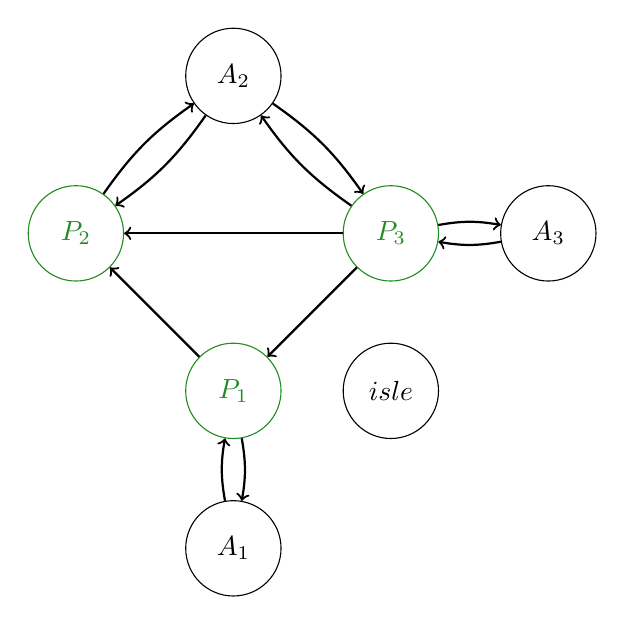
\begin{tikzpicture}[vertex/.style={draw,circle,minimum width=8ex}, arr/.style={draw,thick,->}]
    \node[vertex, color=ForestGreen] (pone) at (0,-2)  {$P_1$};
    \node[vertex, color=ForestGreen] (ptwo) at (-2,0) {$P_2$};
    \node[vertex, color=ForestGreen] (pthree) at (2,0) {$P_3$};
    \node[vertex] (pfour) at (2,-2) {$isle$};
    \node[vertex] (aone) at (0,-4) {$A_1$};
    \node[vertex] (atwo) at (0,2) {$A_2$};
    \node[vertex] (athree) at (4,0) {$A_3$};

    \draw[arr] (pone) -- (ptwo);
    \draw[arr] (pthree) -- (ptwo);
    \draw[arr] (pthree) -- (pone);
    \draw[arr] (athree) to[out=190, in=-10] (pthree);
    \draw[arr] (pthree) to[out=10, in=170] (athree);

    \draw[arr] (aone) to[out=100, in=-100] (pone);
    \draw[arr] (pone) to[out=-80, in=80] (aone);

    \draw[arr] (atwo) to[out=-125, in=35] (ptwo);
    \draw[arr] (ptwo) to[out=55, in=-145] (atwo);

    \draw[arr] (atwo) to[out=-35, in=125] (pthree);
    \draw[arr] (pthree) to[out=145, in=-55] (atwo);
  \end{tikzpicture}
\end{center}
Running the algorithm without a seed set phase on this graph, i.e. all nodes are
starting nodes for the random walks, would give $isle$ an
osrank of $\frac{R (1-\epsilon_{node})}{n R}$. Note that here $n$ is the number
of nodes in the full graph. With the seed set phase though, $isle$
will never be visited by the random walks starting from the seed set nodes and receiving a rank of 0.
With $\tau > 0$ $isle$ will not be eligible to receive \textit{osrank} in and thus not included
in the subgraph for the second phase.

\subsubsection{Incremental algorithm}
The following section is work in progress and has not been implemented yet.\\
Instead of recalculating all \textit{osrank}s whenever the graph changes,
this approach only recalculates the ranks for the nodes that are influenced by
the changes. Changes to the graph can be addition or removal of a node or edge.

\begin{enumerate}
\item  \textbf{Adding a node} without any edge has no effect on the ranking
       of other nodes and the new node does not receive any ranking, i.e. adding a node
       has no effect on its own.
       (Note: This is currently under discussion and might also be influenced
       by decisions around the seed set approach. In theory an added node increases
       $n$ and thus influences the \textit{osrank} of all nodes, but if added during the seed set
       phase this isolated node would be not considered for \textit{osrank} in the
       second phase).
\item \textbf{Removing a node} influences the \textit{osrank} of all nodes.
      This is due to the fact that on the one hand
      after the removal the number of random walks is reduced by $R$ and $n$ by
      $1$, on the other hand, all random walks that visited the removed node
This is due to the fact that on one hand, after the removal, the number of random walks is reduced by $R$ and $n$ by $1$, but on the other hand, all random walks that visited the removed node are invalidated.
\item \textbf{Adding/Removing an edge} influences the graph depending on the type
      of edge. For a changed dependency, random walks
      visiting the starting node of the edge are invalidated. For contribution
      and maintenance edges, random walks visiting both the start and end node
      are invalidated due to their bi-directional nature.
\end{enumerate}

If a change is applied, all invalidated random walks are removed and all nodes visited
by them are registered for \textit{osrank} recalculation. The random walks
for each node are filled up to $R$ again and all visited nodes are
registered for recalculation as well.
In the end for each node registered for recalculation, the visits are counted
and the \textit{osrank} is calculated again.

\subsubsection{Combining the seed set phase and the incremental algorithm}
The following section is work in progress and has not been implemented yet.\\
When combining these two approaches, the changes have to be applied to both phases.
We therefore distinguish between the changes that are passed by the ledger which
are applied in the seed set phase and the changes that are passed by the seed set
phase to the second phase. This means that we will have to store two sets of
random walks, one for each phase.

\begin{center}
  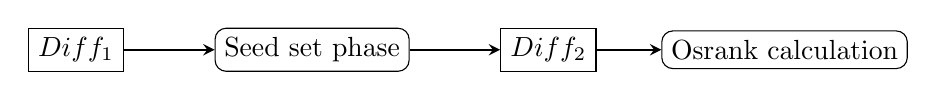
\begin{tikzpicture}[node distance=3cm]
    \tikzstyle{diff} = [draw, rectangle, minimum width=8ex, text centered]
    \tikzstyle{algo} = [draw, rectangle, minimum width=8ex, text centered, rounded corners]
    \tikzstyle{arrow} = [thick,->,>=stealth]
    \node (diff1) [diff] {$Diff_1$};
    \node (seed) [algo, right of=diff1] {Seed set phase};
    \node (diff2) [diff, right of=seed] {$Diff_2$};
    \node (osrank) [algo, right of=diff2] {Osrank calculation};

    \draw [arrow] (diff1) -- (seed);
    \draw [arrow] (seed) -- (diff2);
    \draw [arrow] (diff2) -- (osrank);
  \end{tikzpicture}
\end{center}

$Diff_1$ has the following change events that are similar to the ones described in
the last section with some additions. We distinguish here between simple and seed
set nodes, i.e. nodes are simple as long as they are not in the seed set.
\begin{enumerate}
  \item \textbf{Adding a simple node} has no effect as this event does not add edges. An
  isolated node can't be reached from the seed set.
  \item \textbf{Adding a node to the seed set} increases $n$ and leads to $R$ additional
  random walks. All ranks have to be recalculated. (\textit{Note:} Adding
  the node itself and its edges are different events and precede this event.)
  \item \textbf{Removing a simple node} invalidates all random walks that visited
  this node. In addition all its edges lead to $remove\_edge$ events.
  \item \textbf{Removing a node from the seed set} decreases $n$ and all random
  walks visiting this node are invalidated. All ranks have to be recalculated.
  \item \textbf{Adding an edge} see previous section. (\textit{Todo:} The amount
  of work can potentially be reduced here by analyzing how additional edges actually
  affect the random walks. For example, if both endpoints did not receive rank
  above the threshold before, can the added edge change this?)
  \item \textbf{Removing an edge} see previous section.
\end{enumerate}

$Diff_2$ consists of the following changes:
\begin{enumerate}
  \item The changes from $Diff_1$, if the concerning nodes are eligible for \textit{osrank}
  calculation. The events adding or removing a seed set node are not included in $Diff_2$.
  \item Any node that is newly eligible for \textit{osrank} is included as a $add\_node$
  event. In addition its edges (if both endpoints are eligible for the second phase) are
  included as $add\_edge$ events.
  \item In parallel to the last point, any node that is newly non-eligible for \textit{osrank}
  are included as $remove\_node$ and hence $remove\_edge$.
\end{enumerate}

\subsection{Open questions}
\begin{enumerate}
  \item The model assigns ranks to projects and accounts, but the distribution
  is only meant to be for projects. Should the ranks be normalized again over all
  projects? Which rank will be shown to the user?
  \item Can a project lose its osrank all altogether? (This might happen due to
  the seed set phase)

\end{enumerate}

\section{The Osrank algorithm}

This section describes a possible interface for the \textit{Osrank}
algorithm. If we were to give \textit{Osrank} an abstract
formulation using Rust's traits, a plausible interface could look
like this:

\begin{minted}{rust}
// Definition omitted. The real implementation will likely
// be more complex than this, but somehow it should always
// be possible to get an ID out of either a node or an edge.
trait Graph{
    type NodeId;
    type EdgeId;
}
trait LedgerView{}

trait GraphAlgorithm<'a, G:Graph, L:LedgerView, RNG: 'a> {
    type Input;
    type Output;
    type State;

    /// Access any state necessary for this algorithm to run.
    fn get_state(&self) -> Self::State;
    /// Execute the algorithm.
    fn execute(self, graph: &G, ledger: &L, input: &Self::Input) -> Self::Output;
}
\end{minted}

Assuming the existence of a sound implementation for
the \texttt{Graph} and \texttt{LedgerView} traits,
the \textit{Osrank} implementation could then look like this:

\begin{minted}{rust}
enum MockGraph { MockGraph }
enum MockLedger { MockLedger }
enum Osrank{ Osrank }
type CachedRandomWalks = ();

impl Graph for MockGraph {
    type NodeId = ();
    type EdgeId = ();
}

/// What's changed in the `Graph` respect to the previous invocation of the
/// algorithm.
enum GraphDiff<'a, G: Graph + 'a> {
    NodeAdded(&'a G::NodeId),
    NodeRemoved(&'a G::NodeId),
    EdgeAdded(&'a G::EdgeId),
    EdgeRemoved(&'a G::EdgeId)
}

/// A simplified walk, which implementation is likely to be a bit more
/// complicated than this.
struct Walk<'a, G: Graph + 'a> { walk: Vec<&'a G::NodeId> }

/// A type isomorphic to patch theory edit (See:
/// http://hackage.haskell.org/package/patches-vector-0.1.5.4/docs/Data-Patch.html#t:Edit)
enum WalksDiff<'a, G: Graph + 'a> {
    /// A new walk has been added.
    WalkAdded(&'a Walk<'a, G>),
    /// The walk at index `usize` has been removed.
    WalkRemoved(usize, &'a Walk<'a, G>),
    /// The walk at index `usize` has been replaced.
    WalkReplaced{ position: usize, old: &'a Walk<'a, G>, new: &'a Walk<'a, G> }
}

struct OsrankInput<'a, G: Graph + 'a, RNG> {
    rng: &'a mut RNG,
    graph_diffs: &'a Vec<GraphDiff<'a, G>>
}

struct OsrankOutput<'a, G: Graph + 'a> {
    ranking: RankIterator,
    state_diff: &'a Vec<WalksDiff<'a, G>>
}

struct RankIterator{} //implementation omitted

impl<'a, G: 'a,L,RNG: 'a> GraphAlgorithm<'a, G,L,RNG> for Osrank
where
  L: LedgerView,
  G: Graph  {
    type Input  = OsrankInput<'a, G, RNG>;
    type Output = OsrankOutput<'a, G>;
    type State  = CachedRandomWalks;

    fn get_state(&self) -> Self::State {
        unimplemented!()
    }

    fn execute(self, graph: &G, ledger: &L, input: &Self::Input) -> Self::Output {
      unimplemented!()
    }
}
\end{minted}

Ignoring the dummy types, here are the key ideas:

\begin{enumerate}
\item A source of randomness is provided to the algorithm via
      the \texttt{RNG} type parameter, but it's not a
      requirement for algorithms to use it. In the case of
      \textit{Osrank} though it is indeed needed, so we must
      pass it as an \texttt{Input}.
\item Everything is immutable, including the result, that
      includes some notion of \textit{state difference},
      without actually mutating it.
\item The \texttt{Output} of the \texttt{GraphAlgorithm} could
      also include a data structure that implements the
      \texttt{Iterator} trait, so that upper layer could stream
      the results efficiently. In the example, \texttt{RankIterator}
      is such data structure.
\end{enumerate}

\subsection{The cached random walks}

The \texttt{GraphAlgorithm} trait defines an associated
\texttt{State} type which, in the concrete implementation, is
set to be \texttt{CachedRandomWalks} (for simplicity, aliased
to \texttt{()}). The notion of \textit{random walk} is crucial
in the \textit{incremental Monte Carlo} algorithm
\citep{bahmani10pagerank}, as it's the key to compute the
\textit{Osrank} algorithm efficiently. An initial intuition is
given by the \textit{whitepaper} \citep{opensourcecoin2019}
directly:

"[..]Instead of computing \textit{Osrank} from scratch, we rely
on the fact that only a small percentage of vertices or edges
are added or removed from one calculation to the next. Therefore,
most of the random walks performed in the previous calculation
remain valid in the updated graph[..]".

This is the reason why we introduce the \texttt{GraphDiff}
enumeration: in order to work properly, the \textit{Osrank}
algorithm needs to know, between executions, if the network
graph changed and how, in order to be able to recompute only
the random walks affected.

Defining a precise shape for the \texttt{CachedRandomWalks} might
be outside the scope of this document. What we can do, though, is
to spell out some key characteristics this data structure should
have:

\begin{itemize}
\item Given a \texttt{NodeId} identifying a node $u$, it should
      be possible to efficiently retrieve the \textit{number of visits}
      $X_u$ for the node $u$, i.e. the number of times all the random walks
      visit $u$, in total;
\item Given a now-deleted node $u$ identified by its \texttt{NodeId},
      it should be possible to efficiently retrieve \textit{and
      update} the random walks which visited $u$. This is because now
      any random walk visiting $u$ cannot visit this node anymore, and
      thus the random walk \textit{will} change;
\item Given a newly added edge $(u, v)$, it should be possible to
      efficiently retrieve \textit{and update} all the random walks
      that visits both $u$ and $v$. This is because now any random
      walk passing for $u$ or $v$ could pick this edge, and thus the
      random walk \textit{might} change;
\item Given a now-deleted edge $(u, v)$, it should be possible to
      efficiently retrieve \textit{and update} all the random walks
      that visits both $u$ and $v$. This is because now any random
      walk passing for $u$ or $v$ cannot pick this edge anymore, and
      thus the random walk \textit{might} change;
\end{itemize}

\subsection{Mutating the \texttt{Graph} to recalcutate the weights}

The current trait doesn't allow the \texttt{Graph} to be mutated
during execution, which can be both a good and a bad thing. It's
a good thing as it helps reasoning about the execution and the
algorithm and gives the caller the guarantee that the \texttt{Graph}
won't be modified under the hood, but it's a bad thing as it stops
the algorithm from updating the weights associated to the edges
and to add new nodes to the \texttt{Graph}. There are two obvious
solutions to this:

\begin{enumerate}
\item The \texttt{execute} function should be given a \texttt{\&mut}
      reference to the \texttt{Graph}, so that it can mutate it.
\item The \textit{execution} of the algorithm to compute the rank
      should be separated from the \textit{normalisation} of the
      \texttt{Graph}, which suggests the existence of a function
      to be called before \texttt{execute} that does modify the
      \texttt{Graph}. \footnote{The author is obviously biased by his \textit{Haskell} heritage.}
\end{enumerate}


\subsection{Separating execution from normalisation}

The previous section calls for a separate function which would
mutate an input \texttt{Graph} and perform a number of things:

\begin{enumerate}
\item Update any relevant \textit{weights} for edges which
      were either added or indirectly updated;
\item Normalise the \textit{Graph} so that any parallel
      edges (for example the ones related to contributions,
      maintenance or even project versions) would be collapsed
      in a suitable format for the \textit{Osrank} algorithm,
      which needs to work with only one outgoing edge between
      two nodes;
\end{enumerate}

This could be achieved with another trait, like the following:

\begin{minted}{rust}
trait MutableGraphAlgorithm<'a, G:Graph, L:LedgerView, RNG: 'a>:
  GraphAlgorithm<'a, G,L,RNG> {
    fn normalise(self, graph: &mut G, ledger: &L, input: &Self::Input);
}
\end{minted}

\textbf{There is a big advantage with this approach which might not be
immediately evident}: by separating these two traits, we can ensure
that the \texttt{MutableGraphAlgorithm} stays internal to the
\texttt{Graph API} and/or the \textit{Osrank} project, and the
\texttt{GraphAlgorithm} is exposed to any third-party code wanting
to run computation over a \texttt{Graph} without mutating it.

\subsection{Optimisations}

There are a number of optimizations we can perform over the
original \textit{incremental Monte Carlo} algorithm, in order to
avoid work.

\textbf{1. Ignore disconnected nodes}

If a new node is added, and such node doesn't have any incoming
edges, it means that it cannot be reached from any of the random
walks, \textit{unless} this node is part of the nodes in the
\textit{seed set}. If a node cannot be discovered, it means it
provides no value to the open source ecosystem, and therefore it
shouldn't be entitled to any \textit{oscoin} payment during the
\textit{payout} phase. This translated directly with an
\textit{Osrank} of $0$.

In other terms, if a node is not reachable from one of the
\textit{seed set} vertexes, it can be ignored, and the algorithm
shouldn't be (re)run if such node is added to the graph.

\section{Conclusion}

TBD.

\bibliographystyle{plain}
\bibliography{references}
\end{document}
